\documentclass{article}
\pagenumbering{arabic}
\usepackage{amsmath}
\usepackage{epigraph}
\usepackage{setspace}
\usepackage{float} % Placing tables
\usepackage[showframe=false]{geometry} % Smaller margins
\usepackage{graphicx}
\usepackage{hyperref} % For email addresses
\usepackage[utf8]{inputenc} % Font encoding
\usepackage[parfill]{parskip} % Paragraph formatting
\usepackage[table,xcdraw]{xcolor}
\newcommand{\greytablecell}[1]{\cellcolor[HTML]{DDDDDD}\textbf{#1}}

\begin{document}

\title{

\includegraphics[width=0.2\textwidth]{kthlogo.png}~ 
\\[1cm]
SF2955\\ Computer Intensive Methods In Mathematical Statistics \\Project 1 \\ \Sequential Monte Carlo-based mobility tracking in cellular networks}

\author{Baixi Jin \\ 20000607-T005 \\ \href{mailto:baixi@kth.se}{baixi@kth.se} \and Hanmo Chen \\19990904-T072 \\ \href{mailto:hanmoc@kth.se }{hanmoc@kth.se }}

\date{April 2019}

\maketitle 
\tableofcontents
\newpage


\section{A hidden Markov model for mobility tracking}

\subsection{Motion model}

Consider a target moving in $R^2$, the motion model can be formulated as follows:
\begin{equation}
    \boldsymbol{X}_{n+1}= \boldsymbol{\Phi}\boldsymbol{X}_{n+1}+\boldsymbol{\Psi}_z\boldsymbol{Z}_n+\boldsymbol{\Psi}_{\omega}\boldsymbol{W}_{n+1}
\end{equation}


\subsubsection{$\left\{\boldsymbol{X}_n\right\}_{n\in{N^*}}$ is not a Markov chain} 

According to fundamental Markov property, if the statement holds, $\boldsymbol{X}_{n+1}$ should be conditionally independent of $(\boldsymbol{X}_0,\boldsymbol{X}_1,...)$ given $\boldsymbol{X}_{n}$. However, in this case, ${\boldsymbol{Z}_n}$ is a Markov chain and $\boldsymbol{Z}_{n+1}$ is related with $\boldsymbol{Z}_n$. Thus, $\left\{\boldsymbol{X}_n\right\}$ is not conditionally independent, so it's not a Markov chain.

\subsubsection{$\left\{\tilde{\boldsymbol{X}}_n\right\}_{n\in{N^*}}$ is a Markov chain} 
\begin{equation}
    \tilde{\boldsymbol{X}}_n= (\boldsymbol{X}_n^T,\boldsymbol{Z}_n^T)^T
\end{equation}
First of all, $\left\{\boldsymbol{W}_{n+1}\right\}$ are independent noise variables of $(\boldsymbol{X}_0,\boldsymbol{X}_1,...)$. Secondly, if $\tilde{\boldsymbol{X}}_n$ is given, it means both $\boldsymbol{X}_{n}$ and $\boldsymbol{Z}_{n}$ are known. Since $\boldsymbol{Z}_{n+1}$ only depends on $\boldsymbol{Z}_n$ and is therefore conditionally independent of $(\tilde{\boldsymbol{X}}_0,\tilde{\boldsymbol{X}}_1,...)$,  $\left\{\tilde{\boldsymbol{X}}_n\right\}_{n\in{N^*}}$ is a Markov chain.

\subsubsection{simulation of the trajectory}

We set m=1000. Based on equation (1), the trajectory plot can be obtained.[\ref{1}]

\begin{figure}[h]
        \center{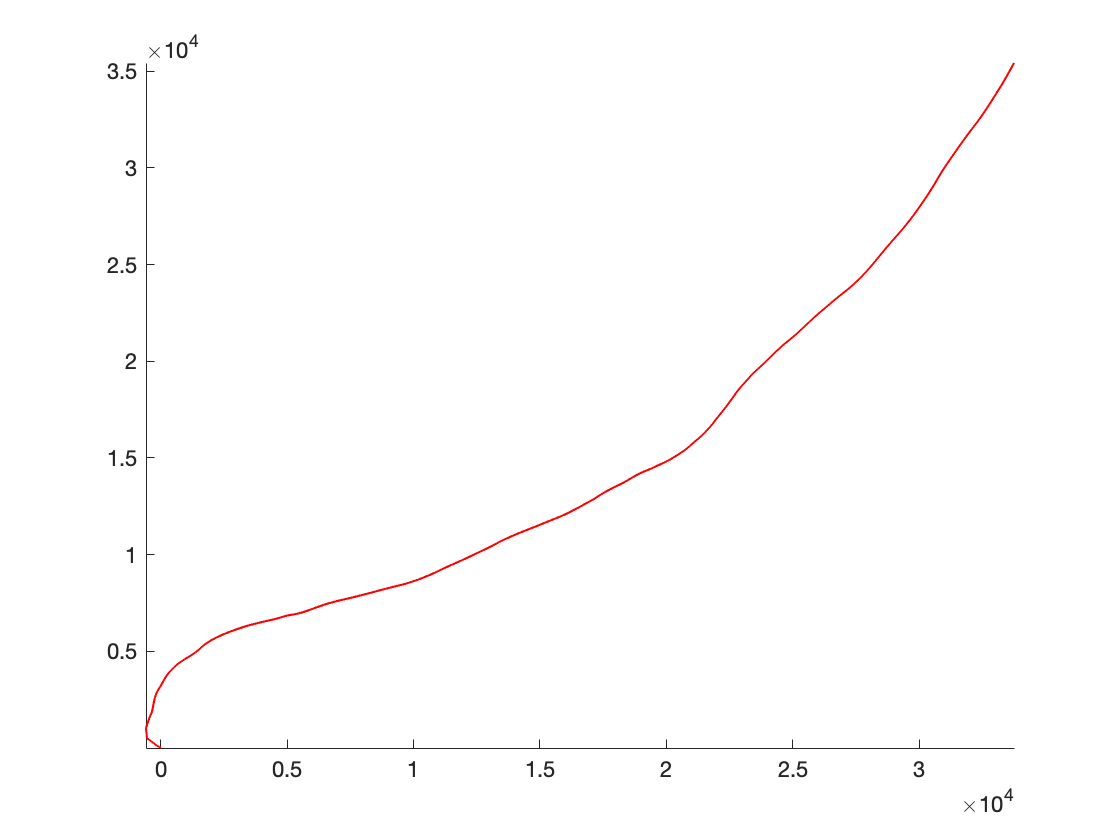
\includegraphics[width=200]{1.png}}
        \caption{\label{1} trajectory of the target under m=1000}
        \end{figure}

\subsection{Observation model}

As the target is moving, it can be detected by received signal strength indication(RSSI) from $s=6$ basic stations(BS). Locations of BS are denoted by $\left\{\boldsymbol{\pi}_l\right\}_{l=1}^s$ and are already known. The RSSI that the mobile unit received from the $l$th BS can be modeled as 
\begin{equation}
    Y_n^l= v-10\eta\log_{10} \left \| (X_n^1,X_n^2)^T-\pi_l \right \|+V_n^l
\end{equation}
where $V_n^l$ are independent Gaussian noises and $v$,$\eta$ are constants. $\left \|\bullet\right \|$ denotes the Euclidean distance.
The RSSIs received at time n from all BSs are denoted by $\boldsymbol{Y}_n=(Y_n^1,...,Y_n^s)^T$.

\subsubsection{$\left\{(\tilde{\boldsymbol{X}}_n,\boldsymbol{Y}_n)\right\}_{n\in{N^*}}$ is a hidden Markov model}
As known before, $\left\{\tilde{\boldsymbol{X}}_n\right\}$ is a Markov chain. But in the observation model, the state $\left\{\tilde{\boldsymbol{X}}_n\right\}$ is not directly visible. However, the output ${\left\{\boldsymbol{Y}_n\right\}}_{n\in{N^*}}$ which is dependent on $\left\{\tilde{\boldsymbol{X}}_n\right\}_{n\in{N^*}}$ is visible. Since $V_n^l$ is independent of time n, $\boldsymbol{Y}_n$ is only dependent on $(X_n^1,X_n^2)$. Thus ${\left\{\boldsymbol{Y}_n\right\}}_{n\in{N^*}}$ are conditionally independent given $\left\{\tilde{\boldsymbol{X}}_n\right\}_{n\in{N^*}}$. i.e.
\begin{equation}
    P(\boldsymbol{Y}_0,\boldsymbol{Y}_1,...|\tilde{\boldsymbol{X}}_0,\tilde{\boldsymbol{X}}_1,...)=P(\boldsymbol{Y}_0|\tilde{\boldsymbol{X}}_0)P(\boldsymbol{Y}_1|\tilde{\boldsymbol{X}}_1)...
\end{equation}
$\left\{(\tilde{\boldsymbol{X}}_n,\boldsymbol{Y}_n)\right\}_{n\in{N^*}}$ is a hidden Markov model.

\subsubsection{The transition density}

\begin{equation}
    p(y_n|\tilde{x_n})=p(y_n|{x_n},z_n)=p(y_n|{x_n})=p(y_n|x_n^1,x_n^2)
\end{equation}
With $(X_m^1,X_m^2)$ given, the only variable left in $y_n$ is $v_n^l$. According to equation (5), 
\begin{equation}
    \boldsymbol{Y}_n^l|\tilde{\boldsymbol{X}}_n \sim\ N(v-10\eta\log_{10} \left \| (X_n^1,X_n^2)^T-\pi_l \right \|,\varsigma^2)
\end{equation}
Hence,
\begin{equation}
    \boldsymbol{Y}_n|\tilde{\boldsymbol{X}}_n \sim\ N(v-10\eta\log_{10} \left \| (X_n^1,X_n^2)^T-\pi_1 \right \|,...,v-10\eta\log_{10} \left \| (X_n^1,X_n^2)^T-\pi_6 \right \|,\varsigma^2\boldsymbol{I}_{6\times6})
\end{equation}

$p(y_n|\tilde{x_n})$ is the density function of the multivariate Gaussian distribution indicated in equation (7).

\section{Mobility Tracking Using SMC Methods} 

Sequential Monte Carlo(SMC) methods can be applied into estimation of positions of the target. Expected positions are denoted by 
\begin{equation}
    \tau_n^1=E[X_n^1|\boldsymbol{Y}_{0:n}=\boldsymbol{y}_{0:n}]
\end{equation}
and \begin{equation}
    \tau_n^2=E[X_n^2|\boldsymbol{Y}_{0:n}=\boldsymbol{y}_{0:n}]
\end{equation}

More specifically, the goal is to produce a sequence $(\tilde{X}_{0:n}^i,\omega_n(\tilde{X}_{0:n}^i))_{i=1}^N$, yet only last particle generation of  $(\tilde{X}_{0:n}^i)_{i=1}^N$ will be used. Since 
\begin{equation}
    \tau_n^i=\int x_n^if(x_n^i| \boldsymbol{y_{0:n}})dx_n^i
\end{equation}
This way, $\tau_n^1$ and $\tau_n^2$ can be approximated.
Sampling from the densities $f(\boldsymbol{\tilde{x}}_n|\boldsymbol{y}_{0:n})$ can be achieved by implementing sequential importance sampling(SIS) and sequential importance sampling with resampling (SISR) algorithms, respectively. 

\subsection{Sequential Importance Sampling (SIS)}
First, we use SIS to sample. In our experiment, the particle sample size N = 10000. In order to obtain better visualization, we have plotted the estimated trajectory of the plane together with locations of basic stations in figure \ref{2}. Obviously, the result is not so satisfying.


\begin{figure}[h]
        \center{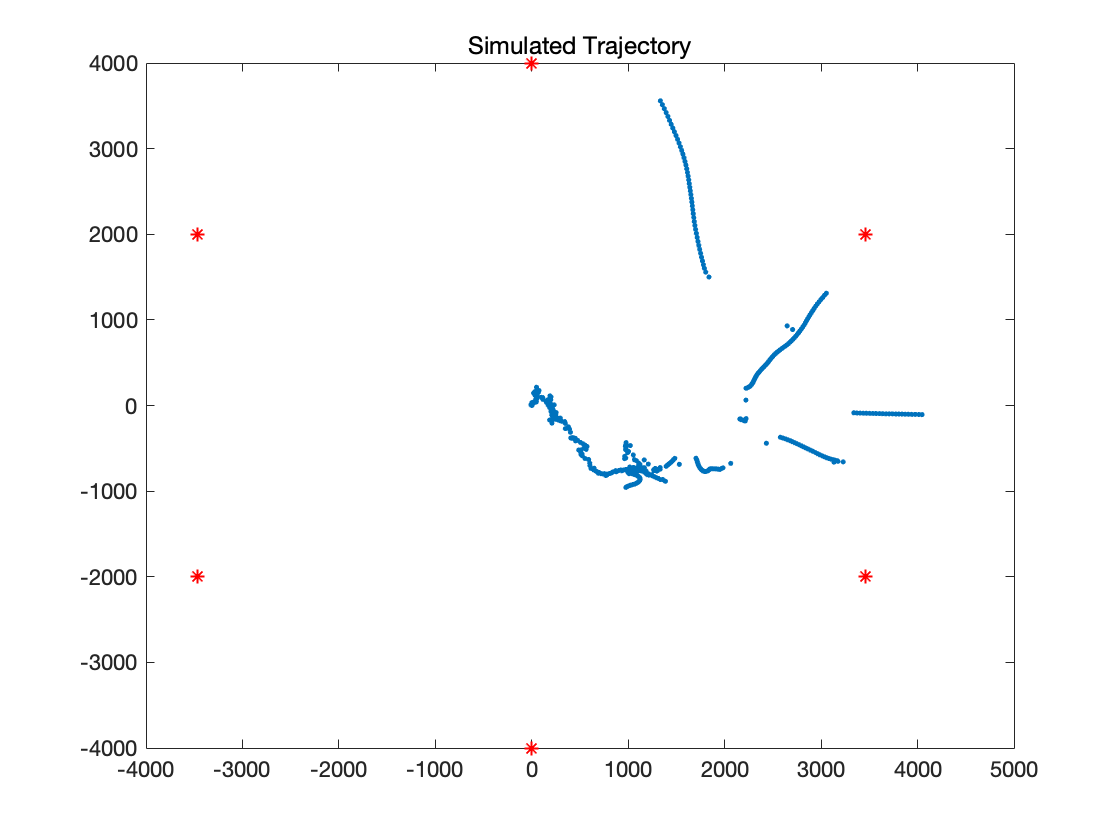
\includegraphics[width=200]{3_1.png}}
        \caption{\label{2} estimates of trajectory of the plane}
    \end{figure}



We have also plotted histograms of the importance weights under n=50, 100 and 200 in figure 3. It is clearly seen that weight degeneration is a universal problem with the SIS method since the weight distribution is skew. 

\begin{figure}[h]
        \center{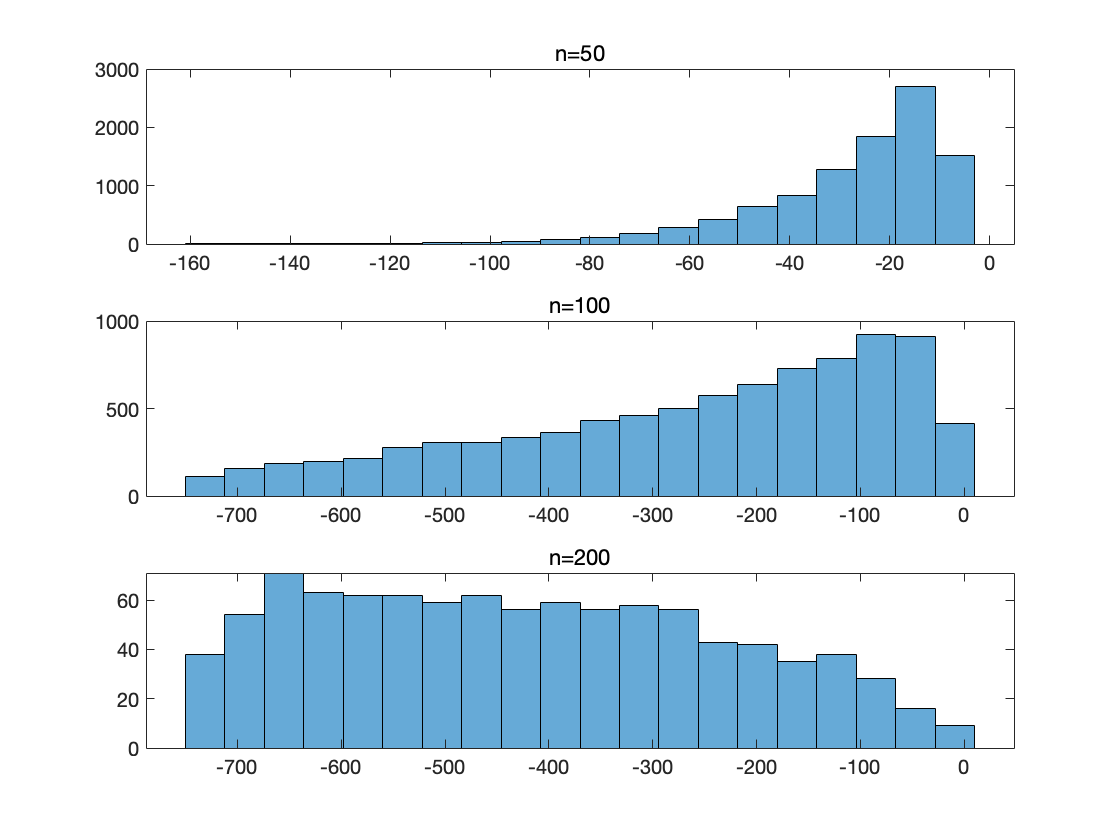
\includegraphics[width=200]{3_2.png}}
        \caption{\label{3} importance weights at n=50, 100, 200}
    \end{figure}

        


The efficient sample size can also be given by $N/(1+CV_n^2)$, where 
\begin{equation}
    CV_n=\sqrt{\frac{1}{N}\sum_{i=1}^N(N\frac{\omega_n^i}{\Omega_n}-1)^2}
\end{equation}

The lower $CV_n$ is, the greater efficient sample size is. The efficient sample sizes at n=50, 100 and 200 are 6227, 2741 and 121, respectively. Figure \ref{4} shows the efficient sample sizes at time points $0:500$.

\begin{figure}[h]
        \center{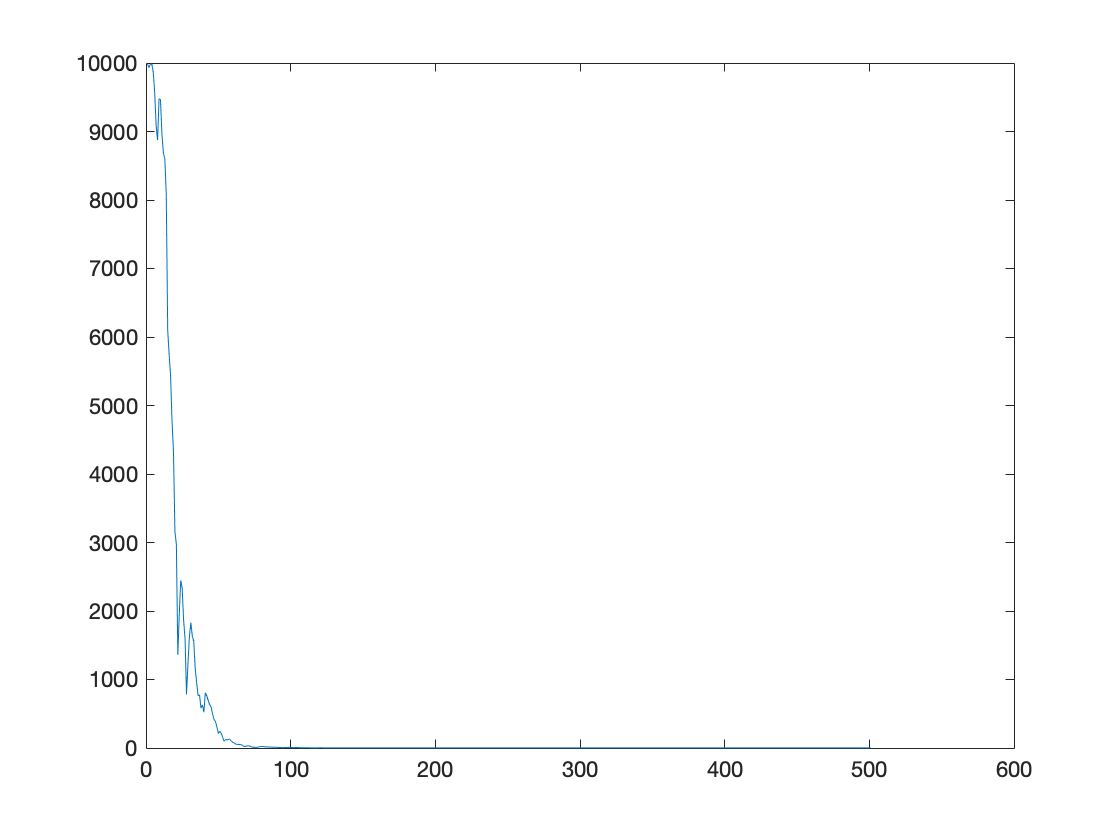
\includegraphics[width=200]{3_3.png}}
        \caption{\label{4} efficient sample sizes at n=0,...,500}
    \end{figure}

\subsection{Sequential Importance Sampling with Resampling(SISR)}
Compared to SIS, we are now implementing SISR algorithm by simply adding a resampling procedure. In our experiment, the particle sample size N = 10000. In order to obtain better visualization, we have plotted the estimated trajectory of the plane together with locations of basic stations in Figure \ref{5}.

\begin{figure}[h]
        \center{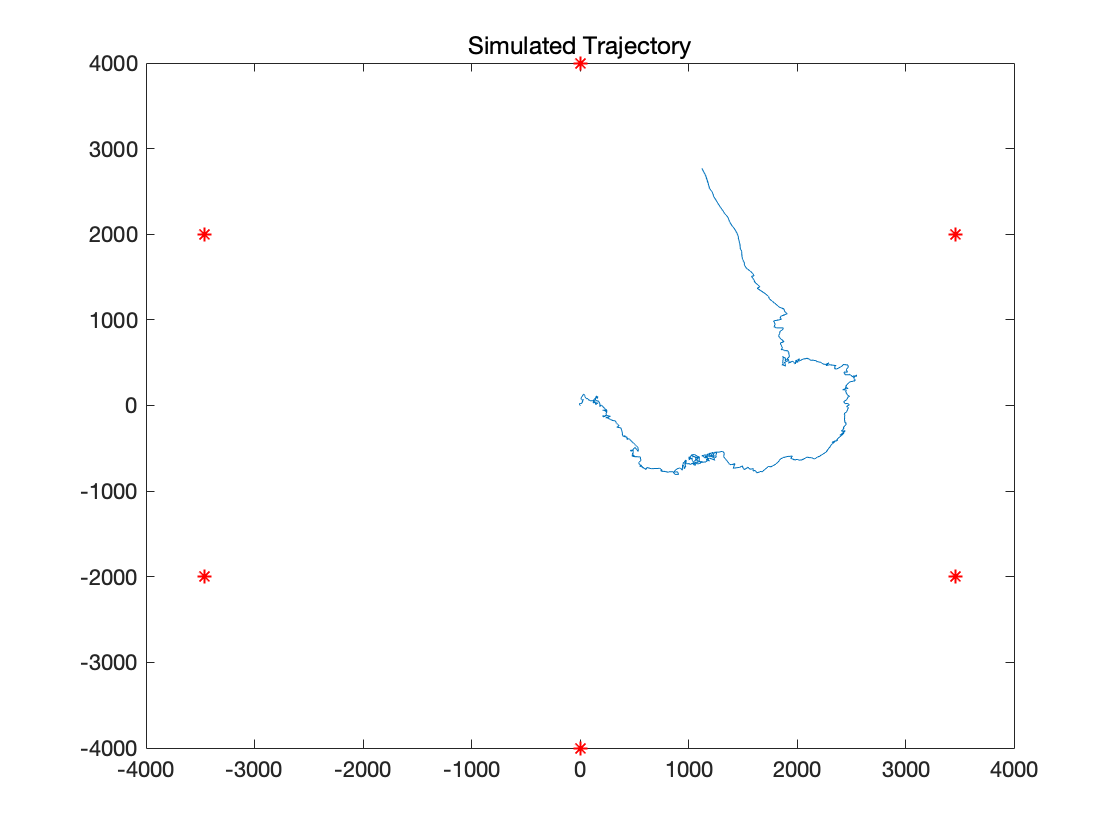
\includegraphics[width=200]{4_1.png}}
        \caption{\label{5} estimates of trajectory of the plane}
    \end{figure}

We have also plotted histograms of the importance weights under n=50, 100 and 200 in Figure \ref{6}. The problem of weight degeneration becomes less severe compared to SIS methods. Among these three time points, n=200 is the best with respect to skewness of weight distribution.

\begin{figure}[h]
        \center{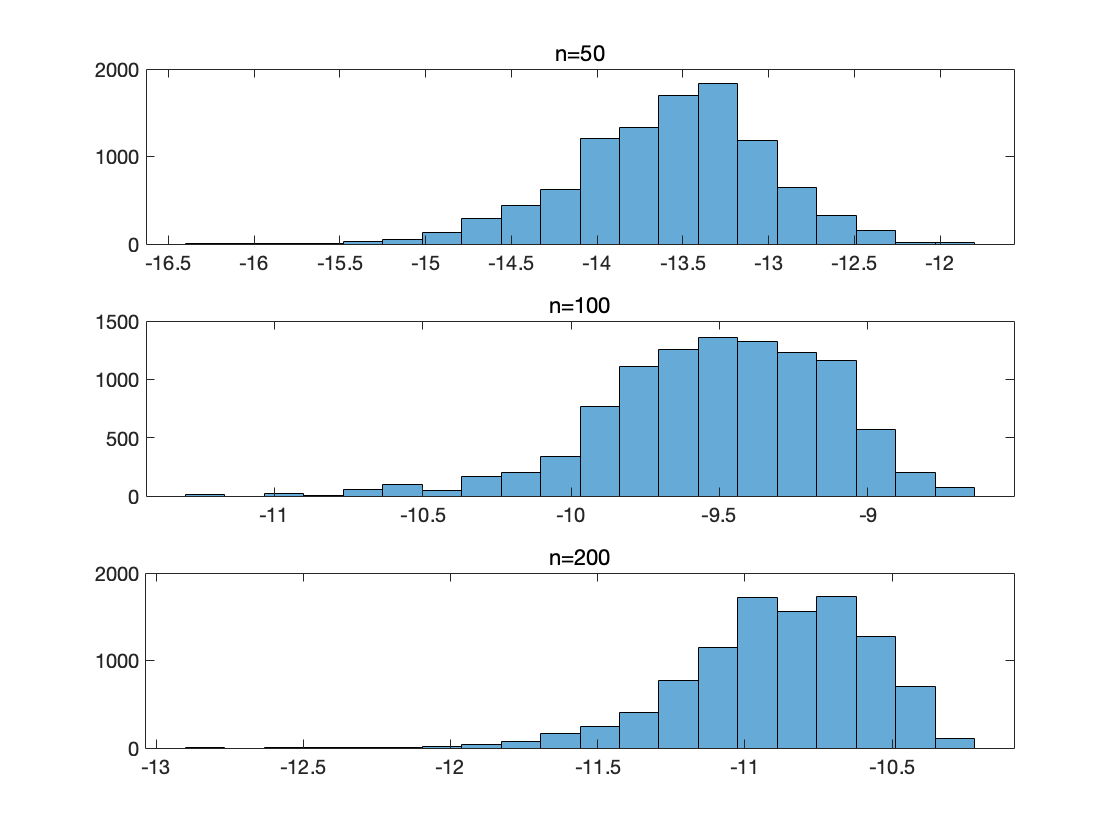
\includegraphics[width=200]{4_2.png}}
        \caption{\label{6} importance weights at n=50, 100, 200}
    \end{figure}
    
The efficient sample sizes at n=50, 100, 200 are 8813, 8670 and 9187, respectively. Figure \ref{7} shows the efficient sample sizes at time points $0:500$.

\begin{figure}[h]
        \center{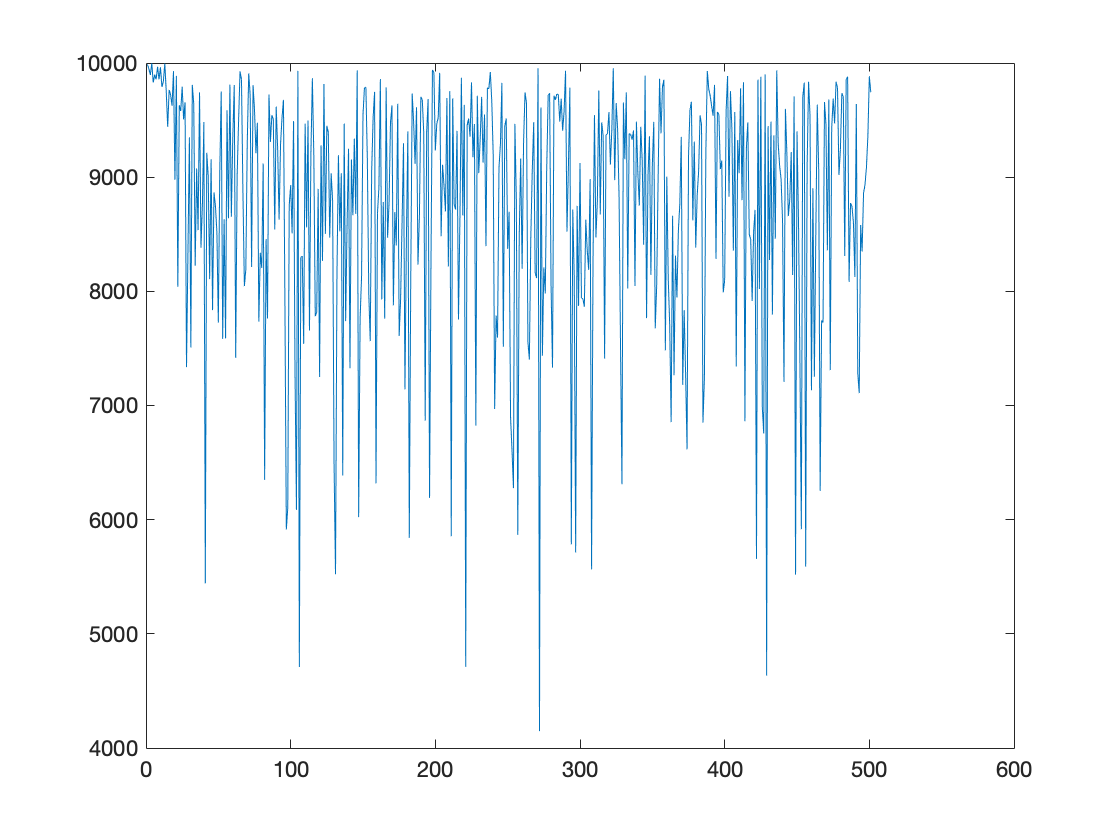
\includegraphics[width=200]{4_3.png}}
        \caption{\label{7} efficient sample sizes at n=0,...,500}
    \end{figure}

\section{SMC-based model calibration}
Assume all parameters except $\varsigma$ are calibrated. We calibrate $\varsigma$ by maximizing the normalized log-likelihood function
\begin{equation}
    \varsigma \mapsto l_m(\varsigma,\boldsymbol{y}_{0:m})=m^{-1}\ln{L_m(\varsigma,\boldsymbol{y}_{0:m})}
\end{equation}
where \begin{equation}
    L_m(\varsigma,\boldsymbol{y}_{0:m})=f_{\varsigma}(\boldsymbol{y}_{0:m})
\end{equation}

In the experiment, we first design the grid $\varsigma_j$ from 0.5 to 3 with increment of 0.05. For each $\varsigma_j$, the SISR algorithm in Problem 4 is implemented and log-likelihood is also estimated. 

\begin{figure}[h]
        \center{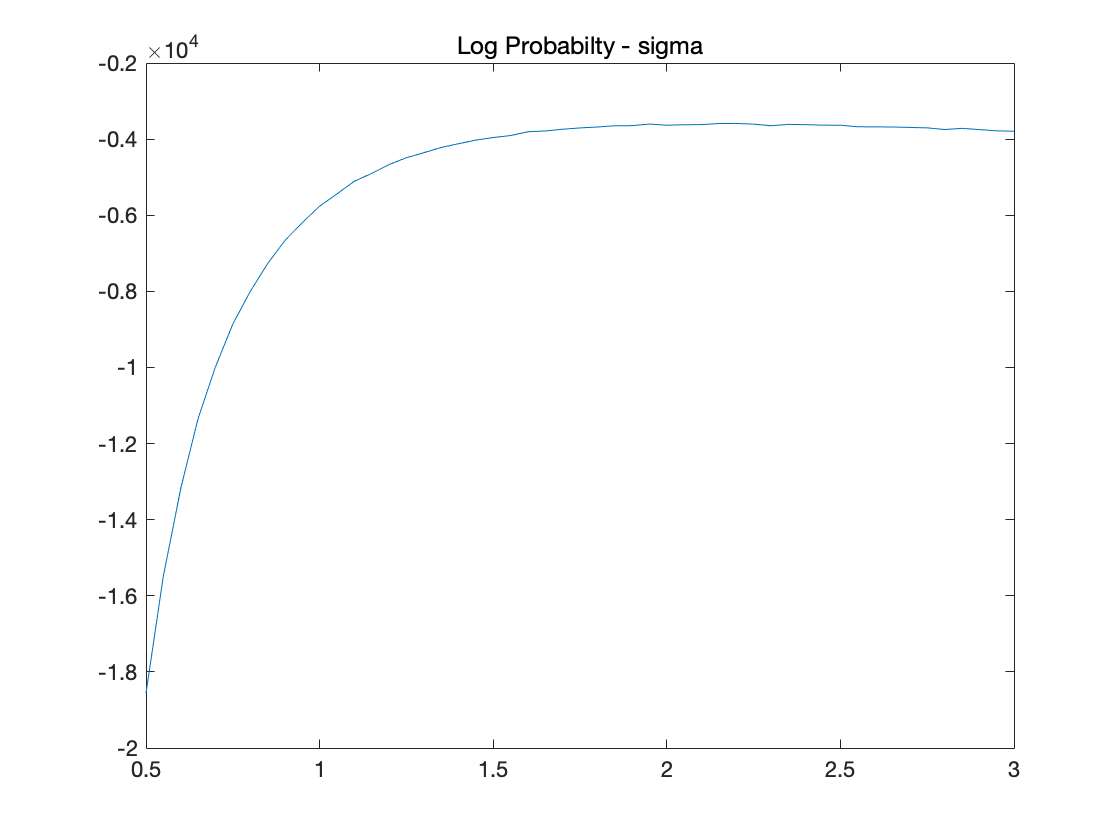
\includegraphics[width=200]{5_1.png}}
        \caption{\label{8} Log Likelihood Estimated}
    \end{figure}

\begin{equation}
    \hat \zeta_m =2.20
\end{equation}
The estimated trajectory under $\hat{\varsigma}_m$ is displayed in Figure \ref{8}.

\begin{figure}[h]
        \center{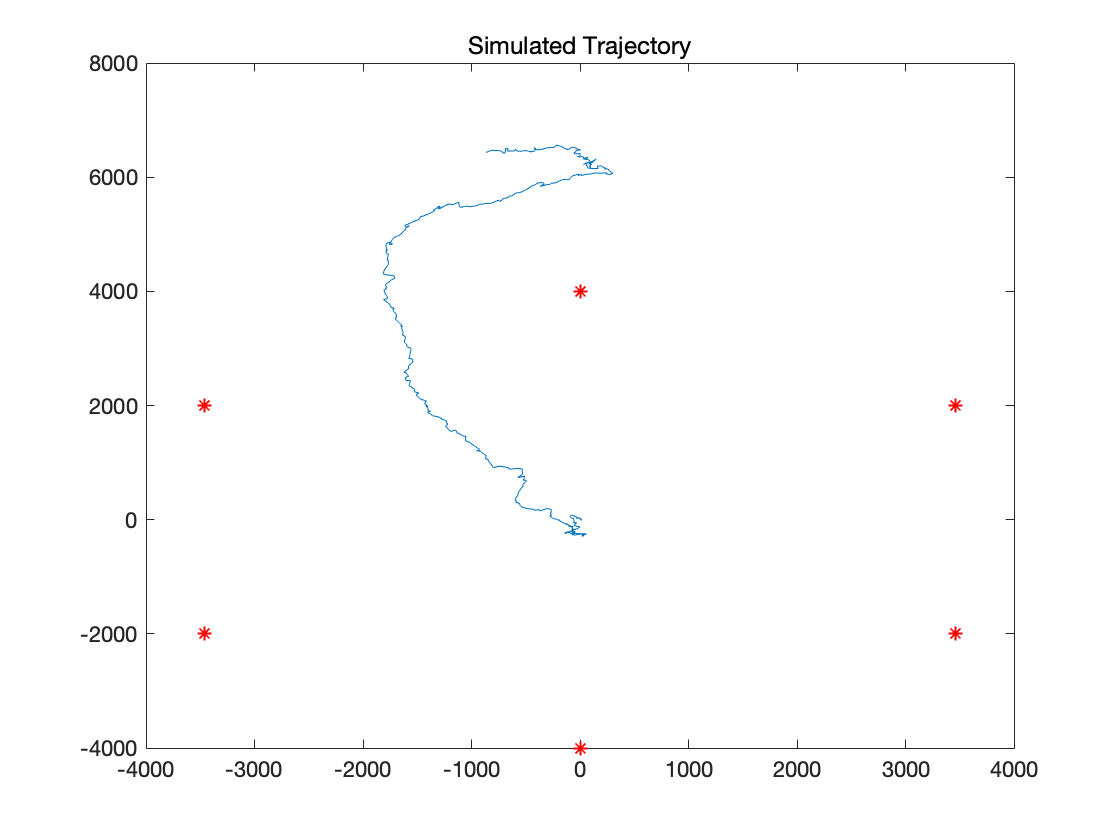
\includegraphics[width=200]{5_2.png}}
        \caption{\label{8} estimates of trajectory of the plane}
    \end{figure}

\end{document}

